\documentclass[10pt,a4paper]{report}
\usepackage[utf8]{inputenc}
\usepackage[portuguese]{babel}
\usepackage{titlesec}
\usepackage{graphicx}
\usepackage{indentfirst}
\usepackage{enumerate}
\usepackage{float}
\usepackage{array}
\usepackage{tikz}
\usepackage{multirow}
\usepackage{multicol}
\usepackage{geometry}
\usepackage{wrapfig}
\usepackage[cache=false]{minted}
\usepackage{pdflscape}
\usepackage[titletoc]{appendix}
\usepackage[hidelinks]{hyperref}
\geometry{
 a4paper,
 top=2cm,
 bottom=2cm,
 left=3cm,
 right=3cm
}
\addto\captionsportuguese{
      \renewcommand{\contentsname}
          {Índice}
}
\titleformat{\chapter}{\normalfont\huge}{\thechapter.}{18pt}{\bf\huge}

\begin{document}
\begin{titlepage}
    \center
    {\huge {\bf Universidade do Minho}}\\[0.4cm]
    \vspace{3.0cm}
    \textsc{\huge{Processamento de xml}}\\[0.5cm]
    \vspace{3.0cm}
    \textsc{\huge{Mestrado Integrado em Engenharia Informática}}\\[0.5cm]
    \vspace{2.0cm}
    \textsc{Laboratórios de Informática 3}\\[0.5cm]
    \textsc{(2º Ano, 2º Semestre, 2017/2018)}\\[0.5cm]
    \vspace{1.5cm}
    \begin{flushleft}
        A79003 \,\,\,Pedro Mendes Félix da Costa
        \vspace{0.2cm}

        A80453 \,\,\,Bárbara Andreia Cardoso Ferreira
    \end{flushleft}
        \vspace{1cm}
    \begin{flushright}
        Braga

        Junho 2018
    \end{flushright}

\end{titlepage}

\tableofcontents
\clearpage

\chapter{Introdução}
    Este trabalho foi feito no âmbito da unidade curricular laboratórios de
    informática 3 e tem como objetivo o processamento de qualquer \textit{dump}
    da base de dados do site \href{www.stackoverflow.com}{StackOverflow} para
    responder a queries de forma eficiente, aplicando conhecimentos de
    algoritemia e programação orientada a objectos.

\chapter{Resolução inicial do Problema}
    Fazendo uma análise às queries, decidimos que seria necessário representar
    as seguintes entidades:

    \section{Posts}
    Para representar um \textbf{Post} criamos a classe abstrata
    do mesmo nome. Esta guarda os dados e representa o comportamento
    comum a todos os posts. Depois, para cada tipo de post considerado, questão
    ou resposta, foi criada uma classe que extende \textbf{Post}, adicionando
    os dados únicos deste tipo.
        \paragraph{Post}
            \begin{multicols}{3}
            \begin{itemize}
                \item Id
                \item Score
                \item Data
                \item Id do autor
                \item Nome do autor
            \end{itemize}
        \paragraph{Questão}
            \begin{itemize}
                \item Título da questão
                \item Número de respostas
                \item Lista das respostas
                \item Tags
            \end{itemize}

        \paragraph{Resposta}
            \begin{itemize}
                \item Número de comentários
                \item Id da questão a que responde
                \item Questão a que responde
            \end{itemize}
            \end{multicols}

    Além dos dados fornecidos diretamente pelos ficheiros xml, decidimos também
    guardar na \textbf{questão} a lista das \textbf{respostas} de cada questão.
    Na \textbf{resposta}, inversamente, guardamos a questão a que esta responde.
    Com estas informações extra, as pesquisas que envolvem relacionar estas duas
    entidades tornam-se muito mais
    eficientes.

    \section{Utilizadores}
    Para representar os \textbf{utilizadores} guardamos os seguintes atributos:
    \begin{multicols}{2}
    \begin{itemize}
        \item Id
        \item Biografia
        \item Nome
        \item Reputação
        \item Número de posts
        \item Lista dos posts
    \end{itemize}
    \end{multicols}
    Mais uma vez foram guardadas mais informações para além das disponibilizadas
    diretamente pelo xml. Foi guardado o número de \textbf{posts} do utilizador
    (para determinar os utilizadores mais ativos de forma mais rápida) e a lista
    destes para permitir pesquisas mais rápidas.

    Esta lista de posts faz uso de uma coleção concebida para resolver este
    tipo de problemas. Neste caso em particular, uma lista ligada ordenada
    (secção \ref{sec:sortedLinkedList}) por data. Devido à forma quase ordenada
    em que os posts surgem no xml esta ordenação é facilmente mantida.


    \begin{figure}[h]
        \centering
        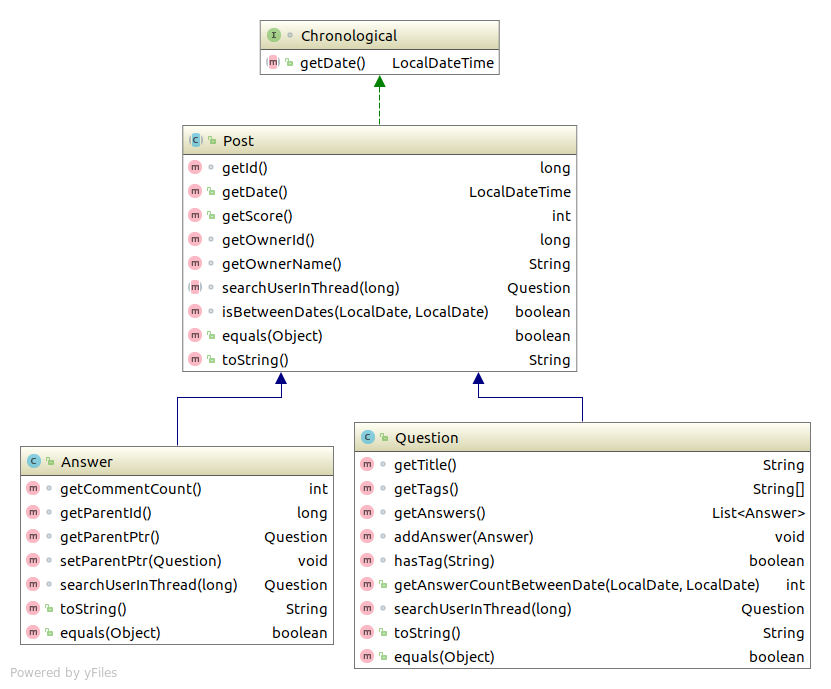
\includegraphics[height=0.4\textheight]{./images/PostHierarchy.png}
        \caption{Hierarquia formada pelos posts}
    \end{figure}

    \begin{figure}[h]
        \centering
        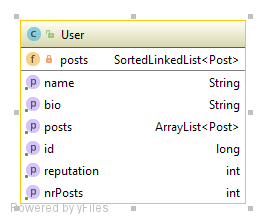
\includegraphics[width=0.4\textheight]{./images/User.png}
        \caption{Classe do utilizador}
    \end{figure}


\chapter{Estruturas de Dados}
    \section{Maps}
        Todas as entidades são armazenadas numa tabela de hash pois para todas
        são necessárias pesquisas por id (ou nome no caso das tags).

        \subsection{Tags}
        A tabela de hash das \textit{tags} serve para criar uma associação
        $Nome \to Id$ visto que as questões guardam uma lista com os nomes das
        tags e para responder à query 11 é necessário obter os ids das mesmas.

    \section{Calendário}
        Para ser possível manter as questões e respostas ordenadas por data foi
        concebida uma estrutura à qual demos o nome de \textbf{Calendário} que
        permite acessos em tempo constante $O(1)$ a todos os elementos
        associados a uma determinada data. Mantemos assim duas instâncias desta
        estrutura na \textbf{Community}, uma para perguntas e outra para
        respostas.

        Para que esta estrutura fosse genérica criamos também uma interface
        \textbf{Chronological} que tem de ser implementada pelos elementos
        que são adicionandos à estrutura. Esta interface obriga à implementação
        do método \mintinline{java}{LocalDateTime getDate()} para que estes
        possam ser guardados de forma ordenada.

        Assim, esta estrutura permite:
        \begin{itemize}
                \item Guardar qualquer objeto desde que implemente a interface
                      referida anteriormente.
                \item Iterar sobre os seus elementos, dado um intervalo de
                      tempo, por ordem cronológica normal ou inversa, conforme a
                      ordem dos argumentos.
        \end{itemize}

        Para utilizar os métodos de iteração, é necessário, para além do
        intervalo de tempo, passar um \textit{Predicate} que é uma classe que
        implementa a interface funcional do mesmo nome. Esta, define um método
        que será aplicado a todos os elementos do \textbf{Calendario} por ordem
        cronológica, inversa ou não, dependendo da ordem em que as datas são
        passadas para definir o intervalo.

        A estrutura em si consiste num \mintinline{java}{Map} que associa a cada
        data uma lista ordenada dos elementos desse data.

        A utilização de listas ligadas para guardar os elementos de um dia é
        mais eficiente, pois é necessário fazer inserções de forma ordenada,
        que são, em quase todos os casos, feitas à cabeça devido aos posts serem
        inseridos quase cronologicamente. Caso não ouvesse esta certeza, estas
        poderiam ser substituídas por um \mintinline{java}{TreeSet} para que
        as inserções fossem no pior caso $O(log(N))$.

    \section{Community}
    Para armazenar as entidades descritas acima foi implementada uma classe
    chamada \textbf{Community} que as armazena de forma a mais tarde facilitar
    as queries que terão de ser feitas sobre estas.

    \begin{figure}[H]
        \centering
        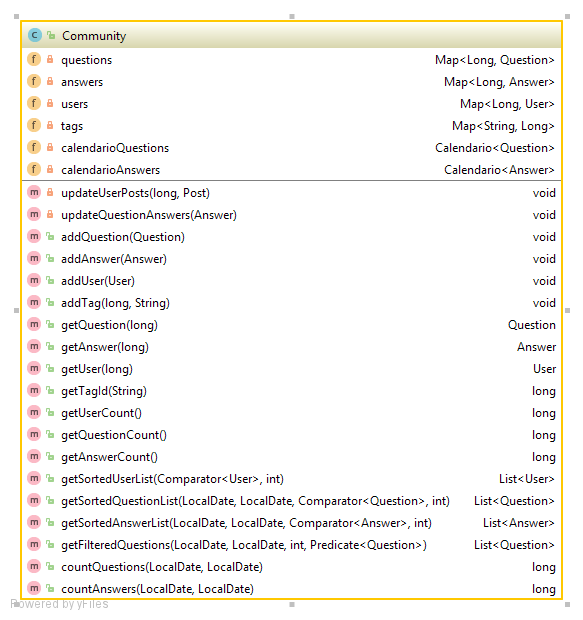
\includegraphics[width=\textwidth]{./images/Community.png}
        \caption{Community}
    \end{figure}

    \section{SortedLinkedList}
    \label{sec:sortedLinkedList}
    Foi necessário desenvolver um novo tipo de lista para satisfazer as
    necessidades de algumas estruturas.
    Esta lista extende \mintinline{java}{LinkedList} adicionando a noção de
    ordem. Para que seja eficiente, esta deve ser usada quando a maior parte
    das inserções forem feitas à cabeça ou na cauda da lista. Opcionalmente,
    esta pode também ter um tamanho máximo.

    \section{TCD}
    A forma como o nosso modelo interage com o exterior é atravez da classe
    \mintinline{java}{TCD}. Esta implementa todas as queries necessãrias de
    forma simples devido à maior parte do processamento ser feito pelos metodos
    disponiveis no \mintinline{java}{Community}.

    \section{Arquitetura}
    Todas estas classes formam a nossa arquitetura que pode ser vista de forma
    esquematizada na Figura \ref{fig:fulldiagram}.

    \begin{figure}[h]
        \centering
        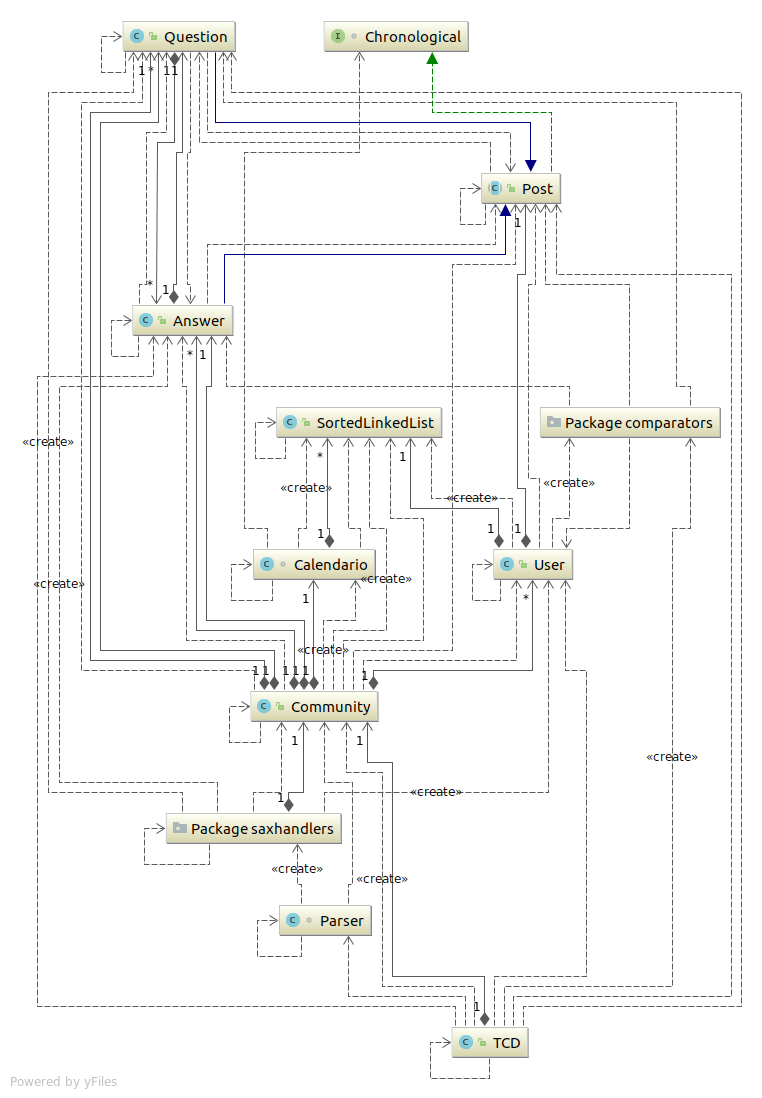
\includegraphics[width=\textwidth]{./images/Model.png}
        \caption{Diagrama de Classes do Engine}
        \label{fig:fulldiagram}
    \end{figure}


\chapter{Modelo MVC e Encapsulamento}
    A arquitetura de packages desenvolvida é a seguinte:
    \begin{itemize}
        \item \textbf{common} Onde estão definidas as classes utilitárias.
        \item \textbf{engine} Onde está definido o modelo.
        \item \textbf{view} Onde está definida a view.
        \item \textbf{li3} Onde está definido o controlador.
    \end{itemize}
    Devido ao uso de packages todas as classes que sejam públicas para fora da
    package, não têm métodos públicos que permitam alterar o seu estado interno.
    Desta forma, todos os objetos aparecem imutáveis para o exterior.

    A \textbf{view} define os métodos para interagir com o utilzador.

    O \textbf{engine} ou \textit{Modelo} define as operações que se podem
    ser realizadas sobre os dados.

    A package \textbf{li3} tem o controlador que faz a comunicação entre os
    pedidos do utilizador e as operações do modelo.

    \begin{figure}[h]
        \centering
        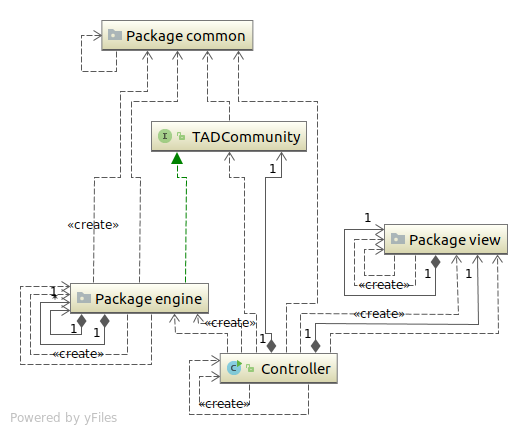
\includegraphics[width=\textwidth]{./images/Top-LevelPackage.png}
        \caption{Diagrama MVC}
    \end{figure}

\chapter{Modularização Funcional e Resolução das queries}
    Para aceder aos dados da estrutura principal foi definida uma API
    simples que permite:
    \begin{enumerate}[1.]
        \item Pesquisas por id de \textbf{questões}, \textbf{respostas} e
        \textbf{utilizadores}.
        \item Pesquisas de ids de \textbf{tags} dada a designação.
        \item Pesquisa de listas, ordenadas por qualquer critério, de
        \textbf{utilizadores}, \textbf{questões} e \textbf{respostas}.
        \item Pesquisas de \textbf{questões} filtradas por qualquer critério.
        \item Contagens de \textbf{questões} ou \textbf{respostas}
              num determinado intervalo de tempo.
    \end{enumerate}

    Com estas funções a resolução da maioria das queries mostrou-se
    trivial.

    Para as queries que necessitam de pesquisas por id (queries: 1, 5, 9 e 10)
    são resolvidas por \textbf{1}.

    Para as queries que necessitam de pesquisas de utilizadores ordenados
    (queries: 2 e 11) são conseguidas através de \textbf{3}, sendo que assim
    basta fornecer um comparator para definir o critério de ordenação.

    Para as queries que necessitam de pesquisas de
    \textbf{perguntas}/\textbf{respostas} num intervalo de tempo ordenadas
    (queries: 6 e 7) são também resolvidas através de \textbf{3}. No caso de não
    ser necessária a filtragem do intervalo de tempo, simplesmente passamos as
    datas máximas disponibilizadas: \mintinline{java}{LocalDate.MAX}
    \mintinline{java}{LocalDate.MIN}.

    Para as queries que necessitam de listas de questões que obedeçam a um
    determinado critério (queries: 4 e 8), são conseguidas através de
    \textbf{4}.

    Para obter o numero de \textbf{perguntas} e \textbf{respostas} dentro
    de um intervalo de tempo (query: 3) fizemos uso dos metodos desenvolvidos
    para este mesmo proposito \textbf{5}.

    A resolução da query 11 tem quatro fases. A primera consiste em obter o top
    N utilizadores (baseado na reputação destes) para para obter os posts
    destes.
    Depois, usando um \mintinline{java}{Map} conta-se a ocorrência de cada
    \textbf{Tag} nas questões dos utilizadores obtidos. Na terceira fase do
    problema, colocam-se as tags numa \textit{PriorityQueue} para que a
    remoção destas seja ordenada por ocorrência, e numa última fase, para cada
    uma das \textbf{Tags} removidas, é adicionado o id desta à lista que será
    retornada.

\chapter{Comparação com a versão em C}
    Em termos de eficiência uma linguagem nativa como C é muito mais rápida a
    executar as queries. Isto notou-se, essencialmente, no parsing.
    \begin{table}[h]
        \centering
        \caption{Comparação de tempos}
        \label{my-label}
        \begin{tabular}{lll}
        \textbf{Query}    & \textbf{C} & \textbf{Java}  \\
        Load              & 10912      & 16827 \\
        Query 1           & 0          & 0     \\
        Query 2           & 25         & 103   \\
        Query 3           & 0          & 1     \\
        Query 4           & 0          & 5     \\
        Query 5           & 0          & 1     \\
        Query 6           & 0          & 6     \\
        Query 7           & 0          & 9     \\
        Query 8           & 0          & 3     \\
        Query 9           & 0          & 1     \\
        Query 10          & 0          & 0     \\
        Query 11          & 22         & 102   \\
        \textbf{Total}    & 11922      & 17058
        \end{tabular}
    \end{table}

    A estrutura que sofreu mais alterações foi o Calendario, inicialmente
    transpilamos o codigo para Java, mantendo a matriz de quatro dimemensões.
    No entanto, quando testamos os tempos das queries verificamos que esta
    não era de forma alguma eficiente, visto que demorava 8000 ms a calcular
    o resultado da query 8. Para resolver este problema desenvolvemos uma
    solução que, no fim, se mostrou relativamente simples.

    Em termos de facilidade de debug e desenvolvimento, o código Java é muito
    mais simples, apesar de não ser uma comparação justa, visto que, tendo o
    trabalho feito em C de forma estruturada, muitos dos possíveis erros já
    foram evitados.

\chapter{Conclusões e Trabalho Futuro}
    Em suma, o grupo considera que o trabalho foi realizado na sua
    totalidade de forma eficiente e correta, respondendo a todas as queries.

    Um aspeto que poderia ser melhorado é a ordenação de utilizadores. Estes
    foram guardados apenas numa tabela de hash, logo, quando é necessária uma
    lista ordenada dos mesmos, a tabela tem de ser percorrida na sua totalidade.
    Esta decisão, centrou-se no facto de que nenhuma única ordenação se
    apresentar particularmente vantajosa, face às demais.

\end{document}
